\subsection{Convolutional Block Attention Module (CBAM)}
By enabling the model to allocate its focus more discriminatively and effectively, the CBAM can potentially aid in learning the most salient features of different pest classes more accurately. This, in turn, may improve the model's ability to distinguish between pests that appear similar or are in different growth stages, thereby enhancing the overall accuracy of the crop pest identification task. So our hypothesis was to integrate CBAM to ResNet architecture to observe the improvement. But addition of CBAM to ResNet architecture didn’t improve the result than it achieved previously.


\subsection{Different growth stage}
In the course of our extensive experimentation, we encountered a significant challenge pertaining to intra-class variation and inter-class similarity of images. The inherent complexity and diversity of visual data led to scenarios where images belonging to the same class displayed stark differences, while images across different classes demonstrated striking resemblances. Such paradoxical occurrences posed a formidable obstacle for each model, as they struggled to accurately categorize certain classes. Consequently, the overall performance of the models fell short of expectations, underscoring the complex and nuanced nature of image classification tasks. It was determined that the primary underlying challenge was the varying growth stages of the pests featured in the images. These different stages introduce additional complexity to the image data, exacerbating the task of class differentiation and thus posing a significant challenge to the modeling process. For example in class 27, peach borer(pest) has 3 different growth stages over the period which makes it difficult for the model to recognize while inference.
\begin{figure}
    \centering
    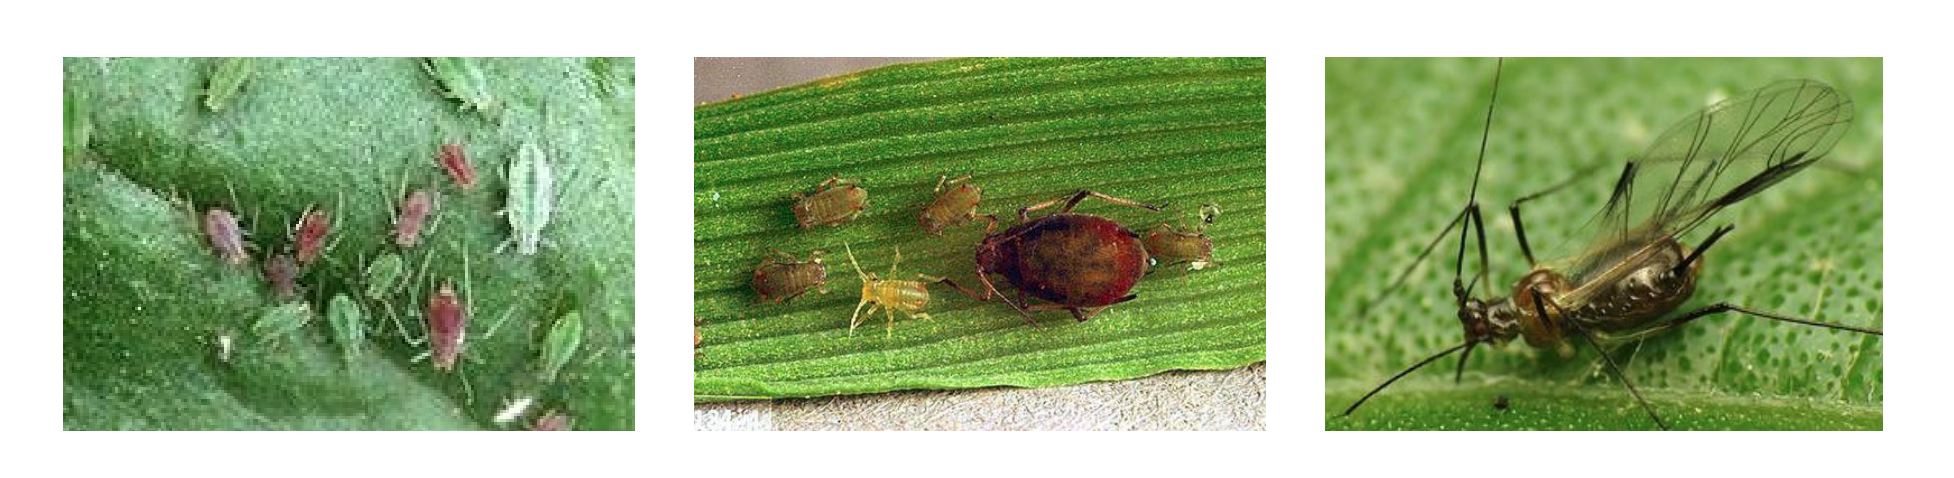
\includegraphics[scale=.4]{figures/Screenshot 2023-05-19 at 5.01.45 AM.png}
    \caption{Result of Focus Region of Interest}
    \label{fig:my_label}
\end{figure}
